\chapter{The Contest Success Function}
\label{ch:model}
\thispagestyle{fancy}

The model my experiment builds upon is inspired by \cite{koch2017} and aims to simulate a process in which an individual competes in several periods to obtain a higher wage in the next period. \cite{koch2017} proposes a Tullock contest in which the relative work supply determines the probability of winning a higher income in the following period and it is described by the Contest Success Function (CSF):

\begin{equation}
    p(x_i,x_{-i}) =
\begin{cases}
    \frac{1}{n},& \text{if } x_i = x_{-i} = 0\\
    \frac{x_i}{x_i + \sum_{j\neq i}^n x_{j}},              & \text{otherwise}
\end{cases}
\label{eq:csf}    
\end{equation}

\hfill \break

Where $x_i$ is the work supplied by participant $i$ and $n$ the total number of participants. So, if a participant provides, for instance, one fourth of the total work supply, she will have a 25 percent chance of obtaining the high income in the following round.\\

Koch's model, however, has several drawbacks. Most notably, that the probability of winning depends only on work supply and therefore redistribution has no direct effect on the Prospect of Upward Mobility. Furthermore, it allows for inequality between players only through the disincentive of taxation (some participants are taxed relatively more because they earn less) but not by differences in ability or outcome. Also, since the contest outcome of one period directly affects the optimal work supply of the next, the best response function and therefore the optimization problem increase in complexity with each round and are not solvable analytically.\\ 

To address those issues I consider a model where the probability of upward mobility is dependant on an individual's relative investment in human capital –similar to investment in private education.\\ 

To be precise, at the end of period $t$, an individual $i$ has the opportunity to invest an amount $I$ of her available income to increase her chances of winning a high income in the next period. Her available income is the income obtained from work after taxation and redistribution. Analogously to the case above, the Contest Success Function (CSF) is therefore defined by:

\begin{equation}
    p(I_i,I_{-i}) =
\begin{cases}
    \frac{1}{n},& \text{if } I_i = I_{-i} = 0\\
    \frac{I_i}{I_i + \sum_{j\neq i}^n I_{j}},              & \text{otherwise}
\end{cases}
\label{eq:csf}    
\end{equation}

\hfill \break

To see how a rational participant would go about deciding her optimal investment, let us consider the simplest case of a game with two periods where the share of total investment at the end of the first period determines the probability of obtaining the prize of a high wage in the second according to the CSF.\\

In the second period, the last in this case, exactly one participant will have a high wage $w_h$ while all others will work with a low wage $w_l$. That means that a participant $i$'s prize, or valuation $\mathbb{V}$ of the game, is equal to the difference in earnings between what she would earn with the high versus with the low wage. At the end of the first period, participant $i$ has then to choose how much to invest in order to maximize the chances of obtaining the prize $\mathbb{V}$.\\

In period 1, a participant wants therefore to maximize her expected profit $\mathbb{E}\Pi_i$ according to the optimization problem:

\begin{equation}
    \underset{I_i}{\text{max}}\quad\mathbb{E}\Pi_i(I_i,I_j) = \frac{I_i}{I_i + \sum_{j\neq i}^n I_{j}}\mathbb{V} - I_i
\label{eq:exp_util}
\end{equation}

Assuming risk-neutrality and that the valuation $\mathbb{V}$ of the higher wage is equal for all participants and therefore that $I_i^{*}=I_{-i}^{*}=I^{*}$ it can be easily shown that the optimal investment amount is\footnote{A step-by-step derivation can be found in the Appendix \ref{ax:derivations}}:

\begin{equation}
    I^{*} = \frac{n-1}{n^2}\mathbb{V}
\label{eq:opt_last}
\end{equation}

\hfill \break 

The optimal amount of investment in the first round will hence depend inversely on the number of participants and directly proportional to the value of the prize.\\

\section{Ensuring Opportunity: The Budget Constraint}
\label{sec:budget_constraint}

But what happens if there are several consecutive rounds? In the presented design, the probability of obtaining the high income in the next period is independent from the previous period only if the optimal investment amount is higher than the available income. In other words, if a participant that has not won the high wage cannot afford the optimal investment, he would have an increased interest to earn the high wage in previous periods. The budget constraint $\frac{n-1}{n^2}\mathbb{V} \leq \pi(w_l)$ is thus violated whenever $\frac{\pi(w_h)-\pi(w_l)}{\pi(w_l)} > \frac{n^2}{n-1}$.\\

Pilot sessions have shown that in a game with three participants, a high wage of approximately five times the low wage will make it impossible for a low wage participant to invest the optimal amount. I take this into account for the current experimental design and make the high wage only twice as large.

\section{Asymmetric Valuations}

An important conundrum that the here presented approach makes easier than \cite{koch2017} to solve is a possible difference in valuation of the prize in terms of higher wage since participants with higher ability or higher utility from consumption will have a higher profit from it. \cite{nti1999} shows that in the two player case:\\

\begin{quote}
    "The player who values the prize more expends more effort in equilibrium but both players allocate the same fraction of their valuations to the contest"\footnote{\cite[p.~419]{nti1999}}.
\end{quote}

To show this, we just need to write the FOC for the two players explicitly\footnote{see the Appendix \ref{ax:derivations} for a derivation of the FOC}:

\begin{equation*}
\begin{split}
    \frac{I_j}{(I_j + I_i)^2}\mathbb{V}_i-1 = 0 \\
    \frac{I_i}{(I_j + I_i)^2}\mathbb{V}_j-1 = 0
\end{split}
\end{equation*}

Equalizing we obtain:
\begin{equation}
    \frac{I_i}{\mathbb{V}_i} = \frac{I_j}{\mathbb{V}_j} 
\end{equation}

Now let us consider the case of $n=3$ for $i \in (a,b,c)$ with exactly one winner\footnote{\cite{stein2002} offers a general derivation for N players}. Using the same process as above we obtain the equation system:

\begin{align}
    \frac{(I_a+I_b)}{(I_a+I_b+I_c)^2}\mathbb{V}_c&=1\\
    \frac{(I_a+I_c)}{(I_a+I_b+I_c)^2}\mathbb{V}_b&=1\\
    \frac{(I_b+I_c)}{(I_a+I_b+I_c)^2}\mathbb{V}_a&=1
\end{align}

To easier visualize the results we assume w.l.o.g that $I_a = I$, $I_b = \beta_b I$ and $ I_c = \beta_c I $, and that $\mathbb{V}_a = \mathbb{V}$, $\mathbb{V}_b = \alpha_b \mathbb{V} $ and $\mathbb{V}_c = \alpha_c \mathbb{V}$. The equation system thus is simplified to:

\begin{align}
    \label{eq:sys1}\frac{(1+\beta_b)}{(1+\beta_b+ \beta_c )^2}\alpha_c\mathbb{V}&=I\\
    \label{eq:sys2}\frac{(1+\beta_c )}{(1+\beta_b  + \beta_c )^2}\alpha_b\mathbb{V}&=I\\
    \label{eq:sys3}\frac{(\beta_b +\beta_c )}{(1+\beta_b  + \beta_c )^2}\mathbb{V}&=I
\end{align}

After setting (\ref{eq:sys2}) = (\ref{eq:sys3}) we obtain:

\begin{equation}
    \label{eq:betab}\beta_b=(1+\beta_c)\alpha_b-\beta_c
\end{equation}

Similarly, we set (\ref{eq:sys1}) = (\ref{eq:sys3}) and obtain $(1+\beta_b)\alpha_c=\beta_b+\beta_c$ in which we can replace $\beta_b$ by (\ref{eq:betab}). Solving for $\beta_c$ we get:
\begin{equation}
\label{eq:betac}
    \beta_c = \frac{\alpha_b-\alpha_c-\alpha_b\alpha_c}{\alpha_b\alpha_c-\alpha_c-\alpha_b}
\end{equation}
Which inserted back in (\ref{eq:betab}) gives us:
\begin{equation}
\label{eq:betab2}
    \beta_b=\alpha_b + \alpha_b\frac{\alpha_b-\alpha_c-\alpha_b\alpha_c}{\alpha_b\alpha_c-\alpha_c-\alpha_b}-\frac{\alpha_b-\alpha_c-\alpha_b\alpha_c}{\alpha_b\alpha_c-\alpha_c-\alpha_b}
\end{equation}

Finally, from (\ref{eq:betab2}) and (\ref{eq:betac}) we know that $\beta_b+\beta_c = 1+\alpha_b\frac{\alpha_b-\alpha_c-\alpha_b\alpha_c}{\alpha_b\alpha_c-\alpha_c-\alpha_b}$ and we can replace in \ref{eq:sys3} to obtain:

\begin{equation}
\label{eq:InvDiffVal}
    I = \frac{\alpha_b+\alpha_b\frac{\alpha_b-\alpha_c-\alpha_b\alpha_c}{\alpha_b\alpha_c-\alpha_c-\alpha_b}}{(1+\alpha_b
    +\alpha_b\frac{\alpha_b-\alpha_c-\alpha_b\alpha_c}{\alpha_b\alpha_c-\alpha_c-\alpha_b})^2}\mathbb{V}
\end{equation}

\hfill \break

Now, to more easily see how this function behaves let us assume that only participant \textit{c} has a different valuation and therefore $\alpha_b = 1$. It follows:

\begin{equation}
    I_a=I_c=\frac{2\alpha_c}{(1+2\alpha_c)^2}\mathbb{V}
\end{equation}

The denominator will grow faster for increasing $\alpha_c$ which means that $I_a$ will tend to $0$.\\


The general case is more cumbersome but we can still find some conditions for the relationship between $\alpha_b$ and $\alpha_c$. Requiring that $\alpha_b, \alpha_c \in \mathbb{R}^+$ and that $\alpha_b\alpha_c-\alpha_c-\alpha_b \neq 0$, it can be shown that, in order for $I\geq0$, then $\alpha_b\alpha_c>\alpha_c+\alpha_b$.\\

This means in particular that there are some levels for which an investment is no longer profitable, take for instance $\alpha_b = 2$ and $\alpha_c = 4$.\\

A look at the function graph \ref{fig:invest_func} gives us a better intuition of its behavior. For very low levels of others' valuations the investment value is close to zero but increases with $\alpha_b$ and $\alpha_c$. After achieving a maximum of $\frac{1}{4}$, or the equivalent to the two player game, the function decreases monotonically.

\begin{figure}[H]
    \centering
    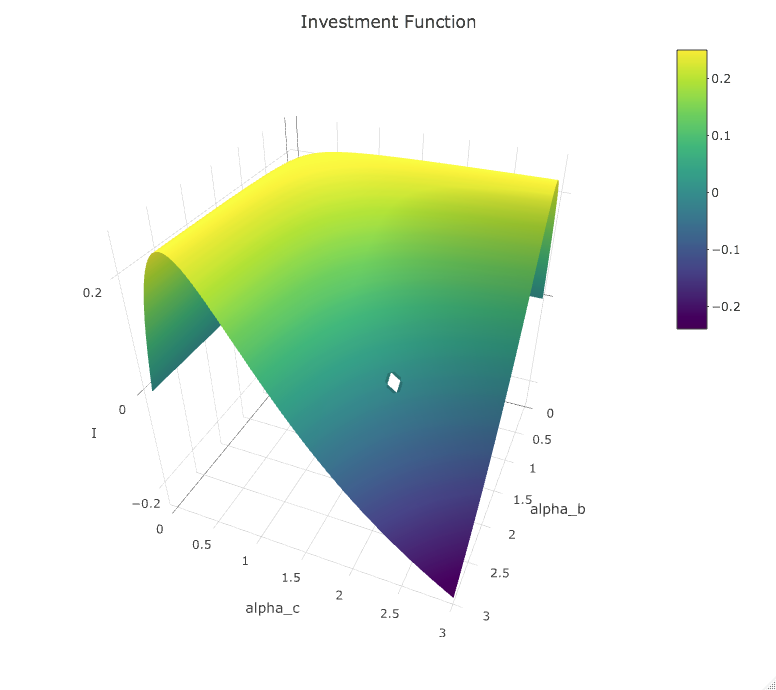
\includegraphics[scale=0.5]{graphs/Investment_Func.png}
    \caption{Investment function dependant on the share of others' valuation}
    \label{fig:invest_func}
\end{figure}

\section{Theoretical Predictions}

Regardless of the repetitions of the game, the expected profit maximizing investment for a given player is constant as shown in equation \ref{eq:opt_last} since, first, the valuation of the game is constant across periods, and, second, the invested amount only affects the winning probabilities of the subsequent period.\\

Furthermore, since work supply does not enter the CSF and, as explained in section \ref{sec:budget_constraint}, participants can always afford to invest their optimum, there is no incentive to work more than the profit maximizing amount.